\chapter{Arhitektura i dizajn sustava}
		
	

	Arhitektura sustava može se podijeliti na tri glavna podsustava:
	
	\begin{itemize}
		\item \textit {Web preglednik} je program koji korisniku omogućuje pregled web stranica i multimedijalnih sadržaja vezanih uz njih. Kada korisnik posjeti neku web stranicu, preglednik preuzima sadržaj sa servera, prilagodi ga, i pokaže ga na zaslonu računala ili nekog drugog uređaja. Korisnik putem web preglednika šalje zahtjev web poslužitelju i dobiva resurse od njega.
		
		\item \textit {Web poslužitelj} je odgovoran za komunikaciju klijenta i web aplikacije. Komunikacija se odvija protokolom za prijenos informacija na webu - HTTP (HyperText Transfer Protocol). Web poslužitelj prima zahtjeve od korisnika putem web preglednika i prosljeđuje ih web aplikaciji na daljnju obradu. Web aplikacija predstavlja središte sustava i obrađuje zahtjeve koje prima od korisnika putem web poslužitelja. Ovisno o zahtjevu, pristupa bazi podataka kako bi dohvatila ili ažurirala podatke. 
		
		\item \textit {Baza podataka} je podsustav za trajnu pohranu podataka koji se koriste u aplikaciji. Web aplikacija komunicira s bazom podataka kako bi dohvatila, ažurirala, brisala ili pohranila podatke prema korisničkim zahtjevima. Podaci se strukturirano pohranjuju i dohvaćaju putem upita. \newline
		
	\end{itemize}
	
		Arhitektura sustava temelji se na MVC (Model-View-Controller) konceptu. Ovaj pristup omogućuje jasnu podjelu odgovornosti unutar sustava, olakšava održavanje, testiranje i proširivost aplikacije. 
		
		\begin{center}
			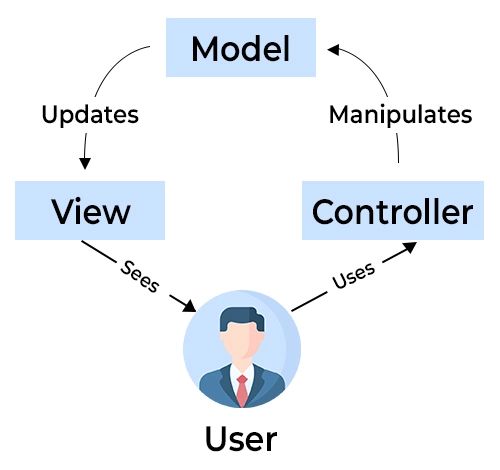
\includegraphics[width=0.4\textwidth]{slike/mvc.png} %veličina u odnosu na širinu linije
		\end{center}
		
		\begin{itemize}
			\item \textit{Model} predstavlja podatke i poslovnu logiku aplikacije. Model je odgovoran za dohvaćanje, pohranu i upravljanje podacima. Komunicira s Controllerom i obavještava ga o ažuriranim informacijama.
			
			\item \textit{View} predstavlja korisničko sučelje aplikacije. Sve što korisnik vidi je dio Viewa. On prikazuje podatke koje dobiva od Modela.
			
			\item \textit{Controller} je posrednik između Modela i Viewa. Prima korisničke zahtjeve iz Viewa, interpretira ih i odabire odgovarajuće akcije. Ovisno o korisničkom zahtjevu, Controller može ažurirati Model (kao što je spremanje podataka u bazu) i/ili ažurirati View (kao što je prikazivanje novih podataka na web stranici). Controller šalje informacije od Viewa prema Modelu, a zatim ažurirane podatke iz Modela šalje natrag Viewu za prikaz korisnicima.
		\end{itemize}
		
		 
		Aplikacija ima slojeve frontend i backend, te bazu podataka. Baza podataka zadužena za pohranu podataka naše web aplikacije je PostgreSQL s kojom smo se upoznali na predmetu Baze podataka. To je moćna relacijska baza podataka koja podržava kompleksne SQL upite i omogućuje efikasno pohranjivanje podataka u tablicama. Osim toga, osigurava konzistentnost i pouzdanost podataka. Iz nje backend sloj dohvaća podatke koristeći radni okvir Spring Boot. Ona olakšava brzi razvoj backenda jer Spring Data JPA omogućuje jednostavno rukovanje podacima putem Java objekata, čime se smanjuje količina potrebnog SQL koda. Također omogućuje lak prijenos podataka između frontend i backend slojeva. Za frontend sloj koji korisnicima prikazuje podatke koje dobiva iz backenda putem API-a koristimo Angular. U kombinaciji sa Spring Boot-om i PostgreSQL-om, Angular je moćni radni okvir koja olakšava izradu modernih, skalabilnih, i korisnički prijateljskih web aplikacija. Temelji se na komponentnoj arhitekturi, što olakšava razdvajanje funkcionalnosti i ponovnu upotrebu koda. Komponente su samostalne i mogu se lako integrirati. Najveća prednost Angulara je što koristi HTML, CSS, te Typescript, jezike koji su poznati svim članovima tima.

		

				
		\section{Baza podataka}
			
			
			
		Za potrebe našeg sustava koristit ćemo relacijsku bazu podataka koja svojom strukturom olakšava modeliranje stvarnog svijeta. Gradivna jedinka baze je relacija, odnosno tablica koja je definirana svojim imenom i skupom atributa. Zadaća baze podataka je brza i jednostavna pohrana, izmjena i dohvat podataka za daljnju obradu.
		Baza podataka ove aplikacije sastoji se od sljedećih entiteta:
		\begin{itemize}
			\item Status
			\item Client
			\item StationLead
			\item Station
			\item Request
			\item Researcher
			\item ActionComment
			\item Action
			\item ExplorerAction
			\item Explorer
			\item ExplorerLocation
			\item AnimalComment
			\item Animal
			\item AnimalLocation
			\item Vehicle
			\item EducatedFor
			\item Task
			\item Token
		\end{itemize}
		
			\subsection{Opis tablica}
				
				\textbf{Status} Ovaj entitet sadržava opis statusa korisnika. Sadrži atribute: statusId i description. Ovaj entitet u vezi je \textit{One-to-Many} s entitetom Researcher preko atributa statusId, u vezi \textit{One-to-Many} s entitetom StationLead preko atributa statusId.
				\begin{longtblr}[
					label=none,
					entry=none
					]{
						width = \textwidth,
						colspec={|X[6,l]|X[6, l]|X[20, l]|}, 
						rowhead = 1,
					} %definicija širine tablice, širine stupaca, poravnanje i broja redaka naslova tablice
					\hline \SetCell[c=3]{c}{\textbf{Status}}	 \\ \hline[3pt]
					\SetCell{LightGreen}StatusId & INT	&  	Jedinstveni identifikator statusa korisnika	\\ \hline
					Description	& VARCHAR &   Opis značenja određenog identifikatora	\\ \hline
				\end{longtblr}
				
				\textbf{Client} Ovaj entitet sadržava korisne informacije o korisniku. Sadrži atribute: clientname, password, photoURL, firstName, lastName, email. Ovaj entitet u vezi je \textit{One-to-One} s entitetom Researcher preko atributa clientname, u vezi \textit{One-to-Many} s entitetom ActionComment preko atributa clientname, u vezi \textit{One-to-One} s entitetom StationLead preko atributa clientname, u vezi \textit{One-to-One} s entitetom Explorer preko atributa clientname.
				\begin{longtblr}[
					label=none,
					entry=none
					]{
						width = \textwidth,
						colspec={|X[6,l]|X[6, l]|X[20, l]|}, 
						rowhead = 1,
					} %definicija širine tablice, širine stupaca, poravnanje i broja redaka naslova tablice
					\hline \SetCell[c=3]{c}{\textbf{Client}}	 \\ \hline[3pt]
					\SetCell{LightGreen}Client & VARCHAR	&  Jedinstveno korisničko ime korisnika  	\\ \hline
					Password	& VARCHAR &   Šifra profila korisnika	\\ \hline 
					PhotoURL & VARCHAR &  URL link slike korisnika \\ \hline 
					FirstName & VARCHAR	&  	Ime korisnika	\\ \hline 
					LastName & VARCHAR	&  	Prezime korisnika	\\ \hline
					Email & VARCHAR	&  	Jedinstveni Email korisnika	\\ \hline
				\end{longtblr}
				
				\textbf{StationLead} Ovaj entitet je razdvojeni entitet entiteta Client koji sadrži atribut poseban za voditelja koji govori koju stanicu vodi (stationId), također sadrži i atribute clientname i statusId. Ovaj entitet u vezi je \textit{One-to-One} s entitetom Client preko atributa clientname, u vezi \textit{One-to-One} s entitetom Station preko atributa stationId, u vezi \textit{Many-to-One} s entitetom Status preko atributa statusId, u vezi \textit{One-to-Many} s entitetom Request preko atributa clientname.
				\begin{longtblr}[
					label=none,
					entry=none
					]{
						width = \textwidth,
						colspec={|X[6,l]|X[6, l]|X[20, l]|}, 
						rowhead = 1,
					} %definicija širine tablice, širine stupaca, poravnanje i broja redaka naslova tablice
					\hline \SetCell[c=3]{c}{\textbf{StationLead}}	 \\ \hline[3pt]
					\SetCell{LightBlue} Clientname	& VARCHAR &   korisničko ime voditelja, (client.clientname)	\\ \hline 
					\SetCell{LightBlue} StationId	& INT &   Identifikator postaje koju voditelj vodi, (station.stationId)\\ \hline 
					\SetCell{LightBlue} StatusId	& INT &   Identifikator statusa profila korisnika (verified, declined, pending), (status.statusId)	\\ \hline 
				\end{longtblr}
				
				\textbf{Station} Ovaj entitet sadržava sve važne informacije o postaji. Sadrži atribute: stationId, radius, stationName, stationStatus, Location. U vezi je \textit{One-to-One} s entitetom StationLead preko atributa stationId, u vezi \textit{One-to-Many} s entitetom Explorer preko atributa stationId.
				\begin{longtblr}[
					label=none,
					entry=none
					]{
						width = \textwidth,
						colspec={|X[6,l]|X[6, l]|X[20, l]|}, 
						rowhead = 1,
					} %definicija širine tablice, širine stupaca, poravnanje i broja redaka naslova tablice
					\hline \SetCell[c=3]{c}{\textbf{Station}}	 \\ \hline[3pt]
					\SetCell{LightGreen}StationId & INT	&  	Jedinstveni identifikator stanice\\ \hline
					Radius	& INT &   Polumjer kruga koji označava stanicu izražen u metrima	\\ \hline 
					StationName & VARCHAR &  Naziv stanice \\ \hline 
					StationStatus & VARCHAR	&  	Status stanice, može biti zauzeta (ima voditelja) ili slobodna (nema voditelja)	\\ \hline 
					Center	& VARCHAR &   Lokacija središta stanice	\\ \hline	 
				\end{longtblr}
				
				\textbf{Request} Ovaj entitet sadržava informacije o zahtjevu koji istraživač šalje voditelju postaje. Sadrži atribute: requestId, status zahtjeva, numOfPeople, researcher i stationLead. U vezi je \textit{Many-to-One} s entitetom Researcher preko atributa researcher, u vezi \textit{Many-to-One} s entitetom StationLead preko atributa stationLead.
				\begin{longtblr}[
					label=none,
					entry=none
					]{
						width = \textwidth,
						colspec={|X[6,l]|X[6, l]|X[20, l]|}, 
						rowhead = 1,
					} %definicija širine tablice, širine stupaca, poravnanje i broja redaka naslova tablice
					\hline \SetCell[c=3]{c}{\textbf{Request}}	 \\ \hline[3pt]
					\SetCell{LightGreen} RequestId	& INT &   Jedinstveni identifikator zahtjeva	\\ \hline
					Status	& VARCHAR &   Status zahtjeva, može biti odobren, odbijen ili u obradi.	\\ \hline
					NumOfPeople & INT &   Broj ljudi koji istraživač zahtjeva od voditelja	\\ \hline
					\SetCell{LightBlue} Researcher	& VARCHAR &   Identifikator istraživača koji šalje zahtjev, (researcher.clientname)	\\ \hline
					\SetCell{LightBlue} StationLead	& VARCHAR &   Identifikator voditelja koji prima zahtjev, (stationLead.clientname)	\\ \hline 
				\end{longtblr}
				
				\textbf{Researcher} Ovaj entitet je razdvojeni entitet entiteta Client koji sadrži atribute: clientname istraživača i statusId. U vezi je \textit{One-to-One} s entitetom Client preko atributa clientname, u vezi \textit{Many-to-One} s entitetom Status preko atributa statusId, u vezi \textit{One-to-Many} s entitetom Request preko atributa clientname, u vezi \textit{One-to-Many} s entitetom Action preko atributa clientname.
				\begin{longtblr}[
					label=none,
					entry=none
					]{
						width = \textwidth,
						colspec={|X[6,l]|X[6, l]|X[20, l]|}, 
						rowhead = 1,
					} %definicija širine tablice, širine stupaca, poravnanje i broja redaka naslova tablice
					\hline \SetCell[c=3]{c}{\textbf{Researcher}}	 \\ \hline[3pt]
					\SetCell{LightBlue}Clientname & VARCHAR	&  korisničko ime istraživača, (client.clientname)\\ \hline
					\SetCell{LightBlue} StatusId	& INT &   Identifikator statusa istraživača (verified, declined, pending), (status.statusId)	\\ \hline 
				\end{longtblr}
				
				\textbf{ActionComment} Ovaj entitet sadrži informacije o komentarima ostavljenima na određenoj akciji. Sadrži atribute: CommentId, description, CommentTS, username i actionId akcije kojoj pripada. U vezi je \textit{Many-to-One} s entitetom Client preko atributa clientname, u vezi \textit{Many-to-One} s entitetom Action preko atributa actionId.
				\begin{longtblr}[
					label=none,
					entry=none
					]{
						width = \textwidth,
						colspec={|X[6,l]|X[6, l]|X[20, l]|}, 
						rowhead = 1,
					} %definicija širine tablice, širine stupaca, poravnanje i broja redaka naslova tablice
					\hline \SetCell[c=3]{c}{\textbf{ActionComment}}	 \\ \hline[3pt]
					\SetCell{LightGreen}CommentId & INT	&  	Jedinstveni identifikator komentara	\\ \hline
					Description	& VARCHAR & Sadržaj komentara	\\ \hline 
					CommentTS & TIMESTAMP &  Vrijeme postavljanja komentara \\ \hline
					Location & VARCHAR &  Lokacija postavljanja komentara \\ \hline 
					\SetCell{LightBlue} Clientname	& VARCHAR &  Identifikator korisnika koji je postavio komentar, (client.clientname)	\\ \hline
					\SetCell{LightBlue} ActionId	& INT &   Identifikator akcije na koju je postavljen komentar, (action.actionId)	\\ \hline 
				\end{longtblr}
				
				\textbf{Action} Ovaj entitet opisuje koji istraživač je pokrenuo određenu akciju. Ima atribute: actionId, researcher, title i description. U vezi je \textit{Many-to-One} s entitetom Researcher preko atributa researcher. U vezi \textit{One-to-Many} s entitetom ActionComment preko atributa actionId, u vezi \textit{One-to-Many} s entitetom ExplorerAction preko atributa actionId, u vezi \textit{One-to-Many} s entitetom Task preko atributa actionId.
				\begin{longtblr}[
					label=none,
					entry=none
					]{
						width = \textwidth,
						colspec={|X[6,l]|X[6, l]|X[20, l]|}, 
						rowhead = 1,
					} %definicija širine tablice, širine stupaca, poravnanje i broja redaka naslova tablice
					\hline \SetCell[c=3]{c}{\textbf{Action}}	 \\ \hline[3pt]
					\SetCell{LightGreen} ActionId & INT	&  	Jedinstveni identifikator akcije  	\\ \hline
					\SetCell{LightBlue} Researcher	& VARCHAR &   Identifikator istraživača koji je započeo akciju, (researcher.clientname)	\\ \hline 
					\SetCell{LightBlue} Title & VARCHAR	&  	Naslov akcije  	\\ \hline
					\SetCell{LightBlue} Description	& VARCHAR &   Opis započete akcije	\\ \hline
				\end{longtblr}
				
				\textbf{ExplorerAction} Ovaj entitet opisuje tragača i akciju na kojoj se nalazio. Ima atribute: explorer i actionId. U vezi je \textit{Many-to-One} s entitetom Explorer preko atributa clientname, u vezi \textit{Many-to-One} s entitetom Action preko atributa actionId.
				\begin{longtblr}[
					label=none,
					entry=none
					]{
						width = \textwidth,
						colspec={|X[6,l]|X[6, l]|X[20, l]|}, 
						rowhead = 1,
					} %definicija širine tablice, širine stupaca, poravnanje i broja redaka naslova tablice
					\hline \SetCell[c=3]{c}{\textbf{ExplorerAction}}	 \\ \hline[3pt]
					\SetCell{LightBlue} Explorer	& VARCHAR &   Korisničko ime tragača, (explorer.clientname)	\\ \hline 
					\SetCell{LightBlue} ActionId	& INT &   Identifikator akcije tragača, (action.actionId)	\\ \hline
				\end{longtblr}
				
				\textbf{Explorer} Ovaj entitet je razdvojeni entitet entiteta Client koji sadrži atribute: clientname i stationId. U vezi je \textit{One-to-One} s entitetom Client preko atributa clientname, u vezi \textit{One-to-Many} s entitetom ExplorerAction preko atributa clientname, u vezi \textit{One-to-Many} s entitetom EducatedFor preko atributa clientname, u vezi \textit{One-to-Many} s entitetom Task preko atributa clientname, u vezi \textit{One-to-Many} s entitetom AnimalComment preko atributa clientname, u vezi \textit{One-to-Many} s entitetom ExplorerLocation preko atributa clientname, u vezi \textit{Many-to-One} s entitetom Station preko atributa stationId.
				\begin{longtblr}[
					label=none,
					entry=none
					]{
						width = \textwidth,
						colspec={|X[6,l]|X[6, l]|X[20, l]|}, 
						rowhead = 1,
					} %definicija širine tablice, širine stupaca, poravnanje i broja redaka naslova tablice
					\hline \SetCell[c=3]{c}{\textbf{Explorer}}	 \\ \hline[3pt]
					\SetCell{LightBlue}Clientname & VARCHAR	&  Korisničko ime tragača, (client.clientname)	\\ \hline
					\SetCell{LightBlue} StationId	& INT &   Identifikator postaje kojoj pripada, (station.stationId)	\\ \hline 
				\end{longtblr}
				
				\textbf{ExplorerLocation} Ovaj entitet sadrži lokaciju tragača u određenom vremenu. Ima atribute: LocationTS, explorer i Location. U vezi je \textit{Many-to-One} s entitetom Explorer preko atributa client.name.
				\begin{longtblr}[
					label=none,
					entry=none
					]{
						width = \textwidth,
						colspec={|X[6,l]|X[6, l]|X[20, l]|}, 
						rowhead = 1,
					} %definicija širine tablice, širine stupaca, poravnanje i broja redaka naslova tablice
					\hline \SetCell[c=3]{c}{\textbf{ExplorerLocation}}	 \\ \hline[3pt]
					\SetCell{LightGreen} Location	& VARCHAR &   Lokacija tragača	\\ \hline
					LocationTS & TIMESTAMP	&  Vrijeme očitanja lokacije tragača\\ \hline
					\SetCell{LightBlue} Explorer	& VARCHAR &   Korisničko ime tragača, (explorer.clientname)	\\ \hline 
					 
				\end{longtblr}
				
				\textbf{AnimalComment} Ovaj entitet sadrži sve komentare o očitanim životinjama. Ima atribute: commentId, commentTS, comment, explorer, animalId. U vezi je \textit{Many-to-One} s entitetom Explorer preko atributa explorer, u vezi \textit{Many-to-One} s entitetom Animal preko atributa animalId.
				\begin{longtblr}[
					label=none,
					entry=none
					]{
						width = \textwidth,
						colspec={|X[6,l]|X[6, l]|X[20, l]|}, 
						rowhead = 1,
					} %definicija širine tablice, širine stupaca, poravnanje i broja redaka naslova tablice
					\hline \SetCell[c=3]{c}{\textbf{AnimalComment}}	 \\ \hline[3pt]
					\SetCell{LightGreen}CommentId & INT	&  Jedinstveni identifikator komentara	\\ \hline
					CommentTS	& TIMESTAMP &   Vrijeme objave komentara	\\ \hline 
					Comment & VARCHAR & Sadržaj komentara  \\ \hline 
					\SetCell{LightBlue} Explorer	& VARCHAR &   Korisničko ime tragača koji je komentirao, (explorer.clientname)	\\ \hline 
					\SetCell{LightBlue} AnimalId	& INT &   Identifikator komentirane životinje, (animal.animalId)	\\ \hline 
				\end{longtblr}
				
				\textbf{Animal} Ovaj entitet sadrži sve bitne informacije o očitanoj životinji. Ima atribute: animalId, species, description, photoURL. U vezi je \textit{One-to-Many} s entitetom AnimalComment preko atributa animalId, u vezi \textit{One-to-Many} s entitetom AnimalLocation preko atributa animalId.
				\begin{longtblr}[
					label=none,
					entry=none
					]{
						width = \textwidth,
						colspec={|X[6,l]|X[6, l]|X[20, l]|}, 
						rowhead = 1,
					} %definicija širine tablice, širine stupaca, poravnanje i broja redaka naslova tablice
					\hline \SetCell[c=3]{c}{\textbf{Animal}}	 \\ \hline[3pt]
					\SetCell{LightGreen}AnimalId & INT	&  	Jedinstveni identifikator očitane životinje  	\\ \hline
					Species	& VARCHAR &   Vrsta životinje	\\ \hline 
					Description & VARCHAR & Opis životinje  \\ \hline 
					PhotoURL & VARCHAR	&  	URL slike životinje	\\ \hline
				\end{longtblr}
				
				\textbf{AnimalLocation} Ovaj entitet sadrži lokaciju životinje u određenom vremenu. Ima atribute: LocationTS, Location, AnimalId. U vezi je \textit{Many-to-One} s entitetom Animal preko atributa animalId.
				\begin{longtblr}[
					label=none,
					entry=none
					]{
						width = \textwidth,
						colspec={|X[6,l]|X[6, l]|X[20, l]|}, 
						rowhead = 1,
					} %definicija širine tablice, širine stupaca, poravnanje i broja redaka naslova tablice
					\hline \SetCell[c=3]{c}{\textbf{AnimalLocation}}	 \\ \hline[3pt]
					\SetCell{LightGreen} Location	& VARCHAR &   Lokacija životinje	\\ \hline
					LocationTS & TIMESTAMP	&  Vrijeme zapisa lokacije životinje	\\ \hline
					\SetCell{LightBlue} AnimalId	& INT &   Identifikator očitane životinje, (animal.animalId)	\\ \hline 
				\end{longtblr}
				
				\textbf{EducatedFor} Ovaj entitet opisuje koji tragači znaju upravljati kojim vozilima. Ima atribute: vehicleId i explorer. U vezi je \textit{Many-to-One} s entitetom Explorer preko atributa clientname, u vezi \textit{Many-to-One} s entitetom Vehicle preko atributa vehicleId.
				\begin{longtblr}[
					label=none,
					entry=none
					]{
						width = \textwidth,
						colspec={|X[6,l]|X[6, l]|X[20, l]|}, 
						rowhead = 1,
					} %definicija širine tablice, širine stupaca, poravnanje i broja redaka naslova tablice
					\hline \SetCell[c=3]{c}{\textbf{EducatedFor}}	 \\ \hline[3pt] 
					\SetCell{LightBlue} VehicleId	& INT &   Identifikator vozila kojeg tragač zna voziti, (vehicle.vehicleId)	\\ \hline 
					\SetCell{LightBlue} Explorer	& VARCHAR &   Korisničko ime tragača, (explorer.clientname)	\\ \hline 
				\end{longtblr}
				
				\textbf{Vehicle} Ovaj entitet sadrži nazive vozila. Ima atribute: vehicleId, vehicleType. U vezi je \textit{One-to-Many} s entitetom Task preko atributa vehicleId, u vezi \textit{One-to-Many} s entitetom EducatedFor preko atributa vehicleId.
				\begin{longtblr}[
					label=none,
					entry=none
					]{
						width = \textwidth,
						colspec={|X[6,l]|X[6, l]|X[20, l]|}, 
						rowhead = 1,
					} %definicija širine tablice, širine stupaca, poravnanje i broja redaka naslova tablice
					\hline \SetCell[c=3]{c}{\textbf{Vehicle}}	 \\ \hline[3pt]
					\SetCell{LightGreen}VehicleId & INT	&  Jedinstveni identifikator vozila	\\ \hline
					VehicleType	& VARCHAR &   Naziv vozila	\\ \hline 
				\end{longtblr}
				
				\textbf{Task} Ovaj entitet sadrži sve bitne informacije o zadatku. Ima atribute: taskId, description, startLocation, endLocation, taskTS, actionId, explorer, vehicleId. U vezi je \textit{Many-to-One} s entitetom Action preko atributa actionId, u vezi \textit{Many-to-One} s entitetom Explorer preko atributa clientname, u vezi \textit{Many-to-One} s entitetom Vehicle preko atributa vehicleId.
				\begin{longtblr}[
					label=none,
					entry=none
					]{
						width = \textwidth,
						colspec={|X[6,l]|X[6, l]|X[20, l]|}, 
						rowhead = 1,
					} %definicija širine tablice, širine stupaca, poravnanje i broja redaka naslova tablice
					\hline \SetCell[c=3]{c}{\textbf{Task}}	 \\ \hline[3pt]
					\SetCell{LightGreen}TaskId & INT	&  	Jedinstveni identifikator zadatka\\ \hline
					Description	& VARCHAR &   Opis zadatka	\\ \hline 
					StartLocation & VARCHAR &  Lokacija početka zadatka \\ \hline 
					EndLocation & VARCHAR	&  	Lokacija završetka zadatka	\\ \hline 
					TaskTS & TIMESTAMP	&  	Vrijeme početka zadatka	\\ \hline 
					\SetCell{LightBlue} ActionId	& INT &   Identifikator akcije kojoj pripada zadatak, (action.actionId)	\\ \hline
					\SetCell{LightBlue} Explorer	& VARCHAR &   Korisničko ime tragača koji izvršava zadatak	\\ \hline 
					\SetCell{LightBlue} VehicleId	& INT &   Identifikator vozila s kojim se obavlja zadatak, (vehicle.vehicleId)	\\ \hline
				\end{longtblr}
				
				\textbf{Token} Ovaj entitet sve podatke o tokenu koji se generira pri registraciji ili prijavi korisnika u sustav. Ima atribute: tokenId, tokenType, revoked, expired, clientname. U vezi je \textit{Many-to-One} s entitetom Client preko atributa clientname.
			     \begin{longtblr}[
					label=none,
					entry=none
					]{
						width = \textwidth,
						colspec={|X[6,l]|X[6, l]|X[20, l]|}, 
						rowhead = 1,
					} %definicija širine tablice, širine stupaca, poravnanje i broja redaka naslova tablice
					\hline \SetCell[c=3]{c}{\textbf{Token}}	 \\ \hline[3pt]
					\SetCell{LightGreen}TokenkId & INT	&  	Jedinstveni identifikator tokena\\ \hline
					TokenType & VARCHAR & Tip generiranog tokena \\ \hline
					Token & VARCHAR & Generirani token \\ \hline
					Revoked & BOOLEAN & Zastavica koja daje informaciju o tome je li token opozvan \\ \hline
					Expired & BOOLEAN & Zastavica koja daje informaciju o tome je li token istekao \\ \hline
					\SetCell{LightBlue} Client	& VARCHAR &   Korisničko ime klijenta koji koristi token, (client.clientname)	\\ \hline
					
				\end{longtblr}
				
				
			
			\subsection{Dijagram baze podataka}
				\begin{figure}[H]
					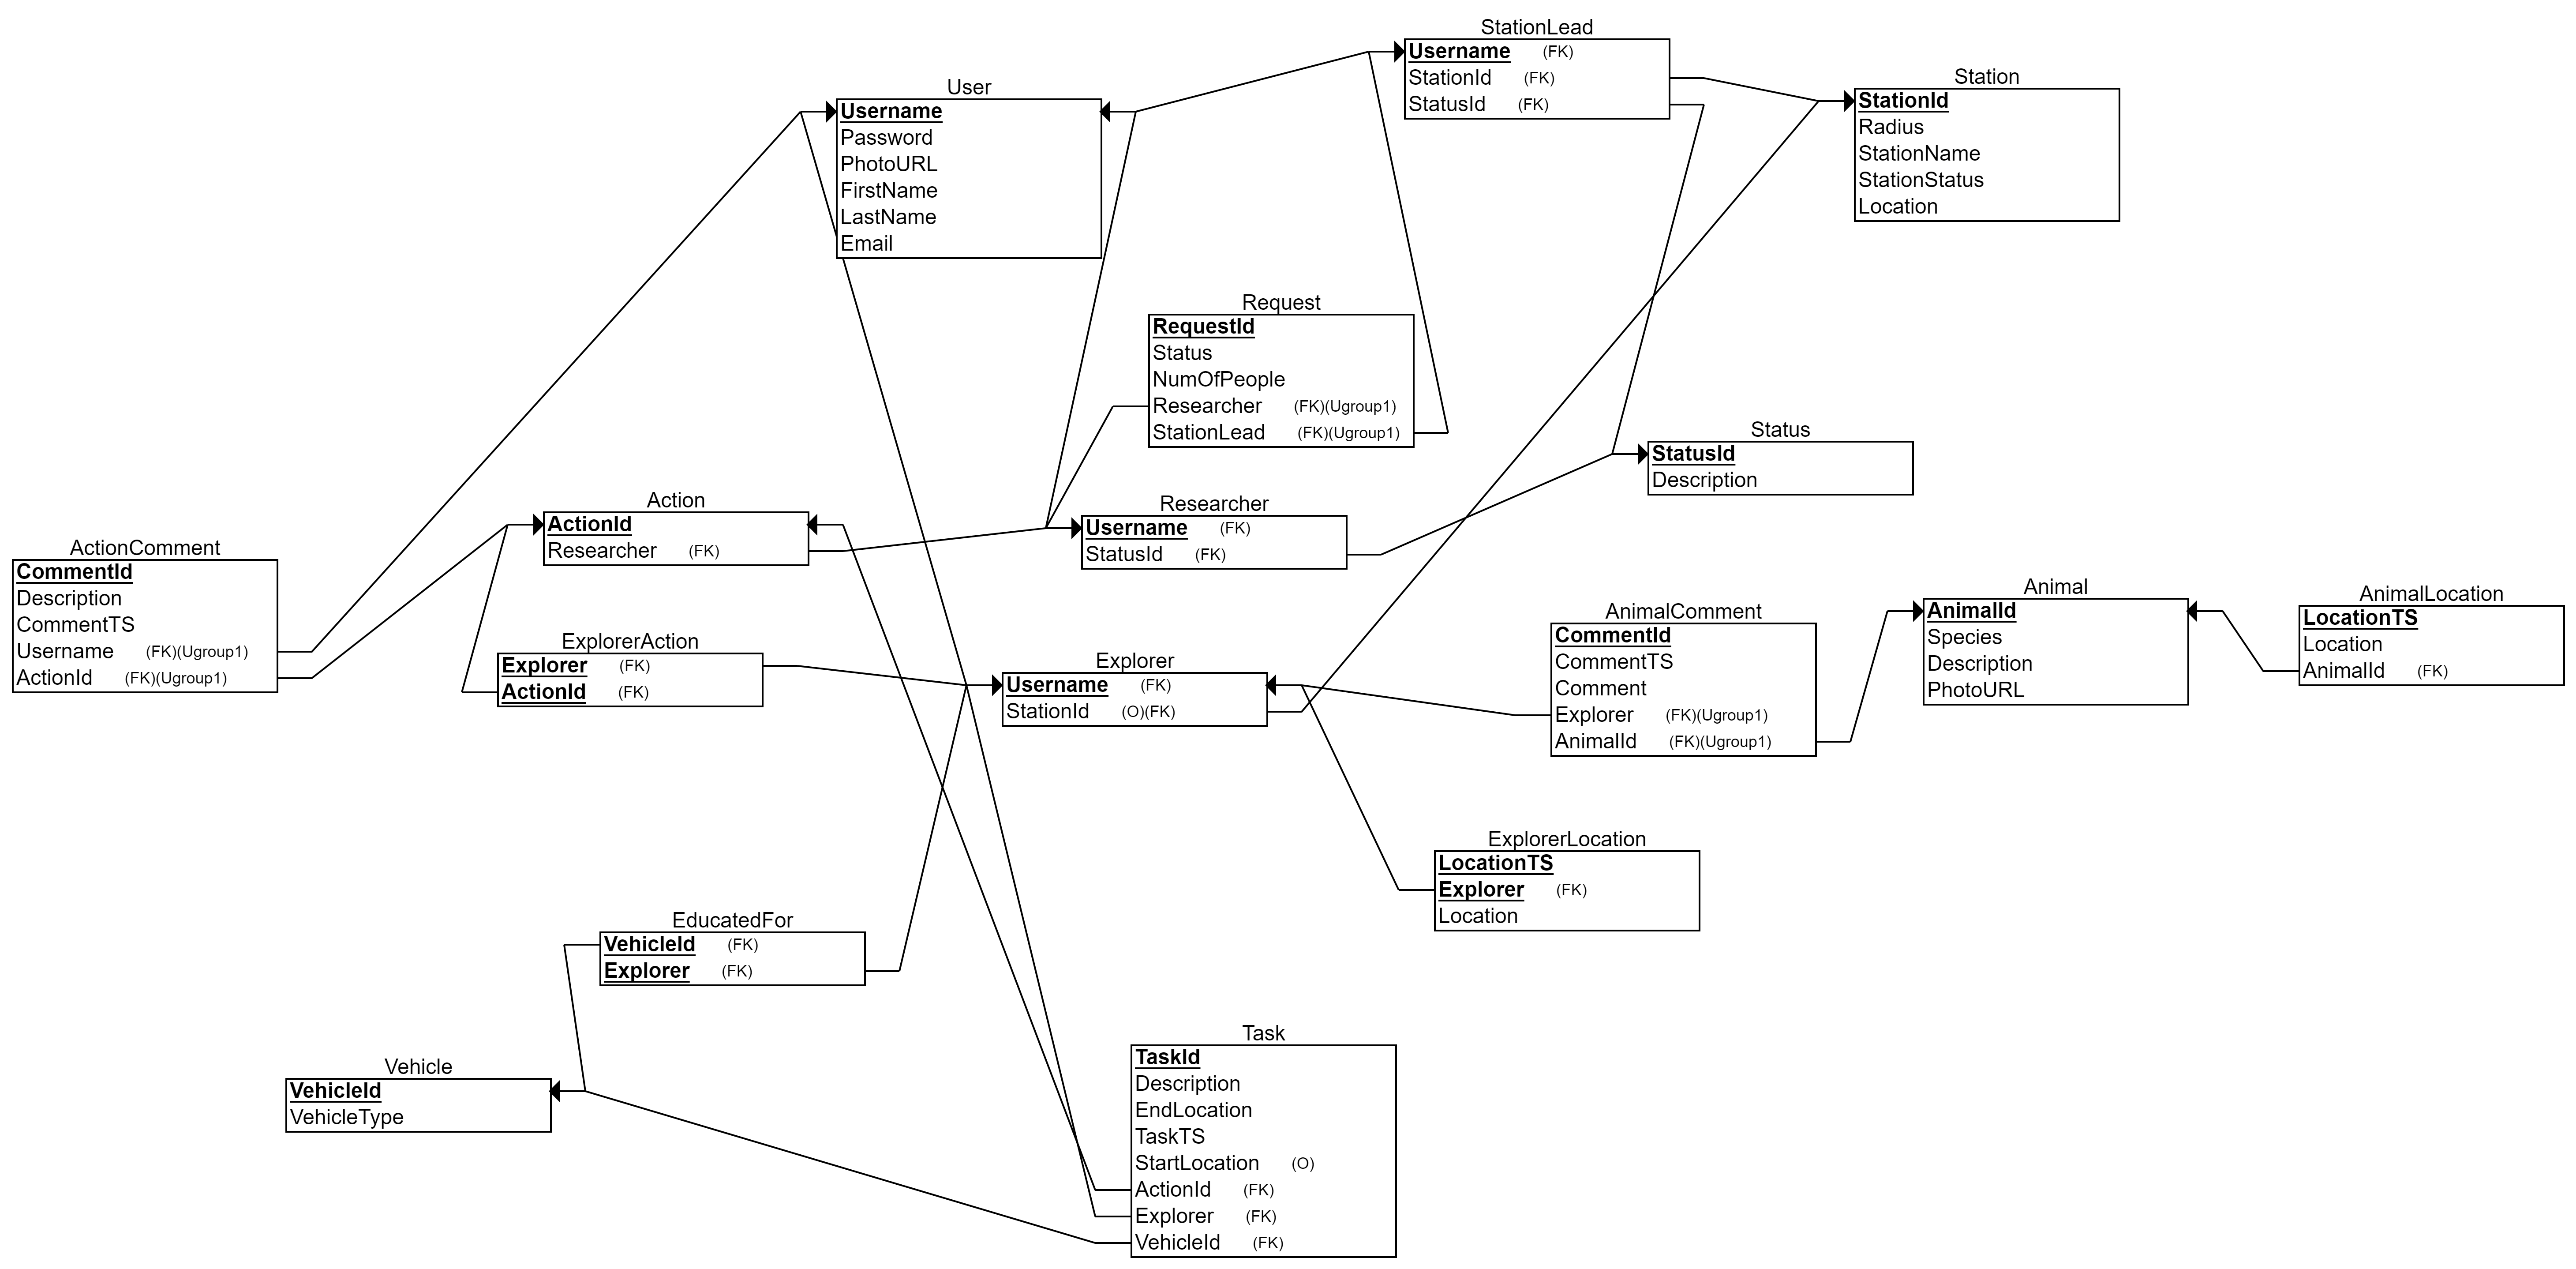
\includegraphics[width=\textwidth]{slike/dijagram_baze.PNG} %veličina u odnosu na širinu linije
					\caption{Dijagram baze podataka}
					\label{fig:dijagram_baze} %label mora biti drugaciji za svaku sliku
				\end{figure}
			
			\eject
			
			
		\section{Dijagram razreda}
		
			Na slikama 4.2, 4.3 predstavljeni su razredi koji se odnose na backend komponentu MVC obrasca. Razredi na slici 4.2 nasljeđuju Controller razred. U tim razredima, metode rukuju s Data Transfer Object (DTO), a podaci se dohvaćaju kroz metode definirane u Model razredima. Funkcije implementirane u Controller razredima generiraju JSON datoteke s HTML status kodovima.S ciljem olakšane organizacije, razredi su strukturirani prema ovlastima određenih korisnika, a unutar dijagrama su predstavljene isključivo povezanosti između razreda unutar istog dijela dijagrama. Iz naziva i tipova atributa u razredima može se zaključiti vrsta povezanosti između različitih razreda.
			
			\vspace{90pt}
			
			
			\begin{figure}[H]
				\centering
				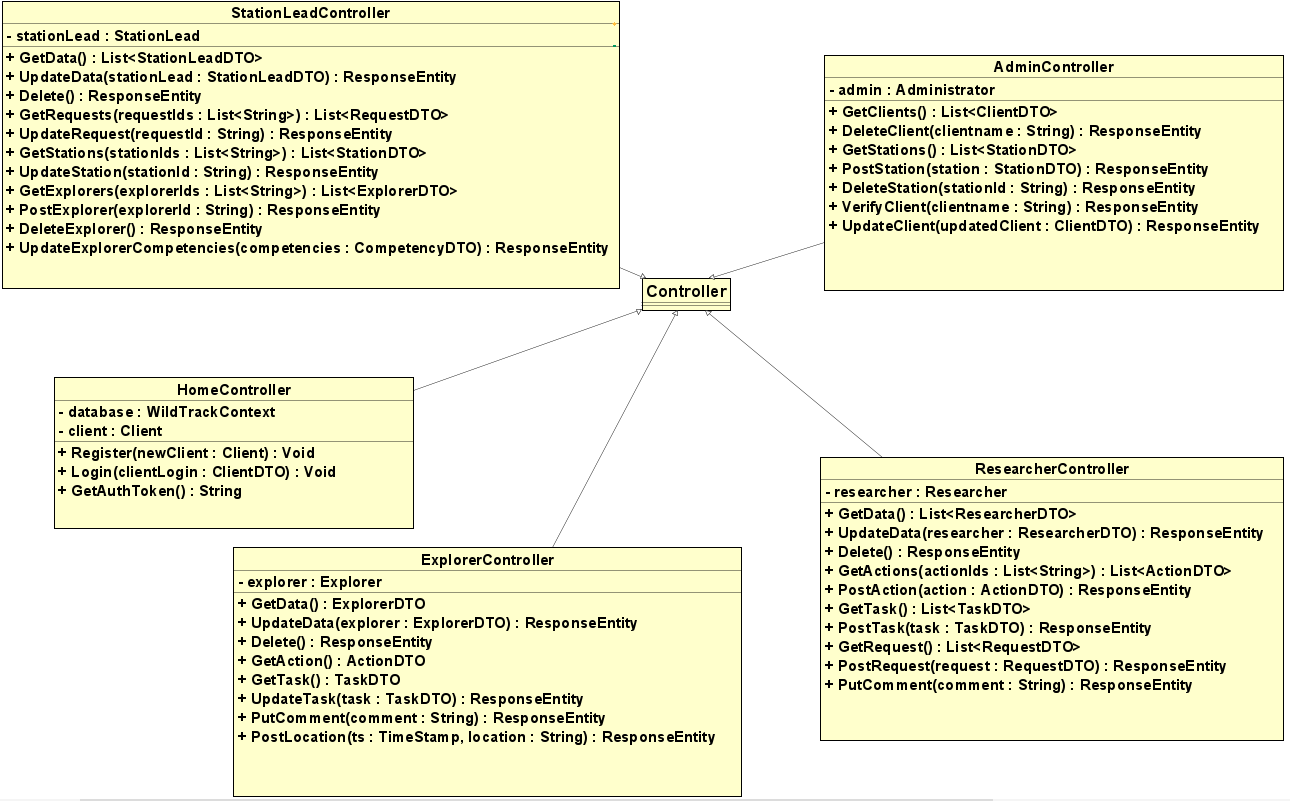
\includegraphics[width=\textwidth]{slike/Controlleri.PNG}
				\caption{Dijagram razreda - dio Controllers}
				\label{fig:dijagram_baze}
			\end{figure}
			
			
			\begin{figure}[H]
				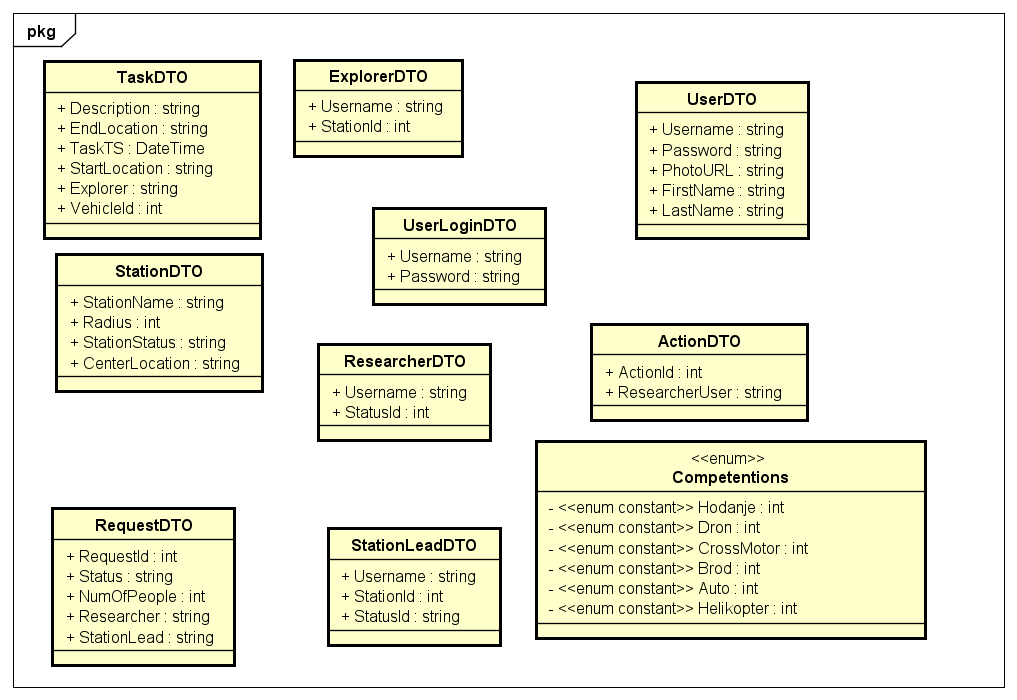
\includegraphics[width=\textwidth]{slike/Class_Diagram0.PNG} %veličina u odnosu na širinu linije
				\caption{Dijagram razreda - dio Data transfer objects}
				\label{fig:dijagram_baze} %label mora biti drugaciji za svaku sliku
			\end{figure}
			
			\vspace{36pt}
			
			Implementirane metode direktno komuniciraju s bazom podataka te vraćaju tražene podatke. Razred User predstavlja neregistriranog korisnika koji se može registrirati u sustav unoseći osnovne informacije. Razred UserLogin predstavlja već registriranog korisnika koji se može prijaviti u sustav unoseći korisničko ime i lozinku. Razred Reasearcher predstavlja istraživača koji ima ovlasti kreiranja novih akcija i slanja zahtjeva za tragačima voditelju postaje. Razred StationLead predstavlja voditelja postaje koji ima ovlasti odabrati postaju i tragače svoje vlastite postaje. Razred Explorer predstavlja tragača koji obavlja zadatke koje mu je dodijelio istraživač. Razred Administrator predstavlja administratora sustava koji ima najveće ovlasti.
			
			\vspace{36pt}
		
		\section{Dijagram stanja}
			
			
			\textbf{\textit{dio 2. revizije}}\\
			
			\textit{Potrebno je priložiti dijagram stanja i opisati ga. Dovoljan je jedan dijagram stanja koji prikazuje \textbf{značajan dio funkcionalnosti} sustava. Na primjer, stanja korisničkog sučelja i tijek korištenja neke ključne funkcionalnosti jesu značajan dio sustava, a registracija i prijava nisu. }
			
			
			\eject 
		
		\section{Dijagram aktivnosti}
			
			\textbf{\textit{dio 2. revizije}}\\
			
			 \textit{Potrebno je priložiti dijagram aktivnosti s pripadajućim opisom. Dijagram aktivnosti treba prikazivati značajan dio sustava.}
			
			\eject
		\section{Dijagram komponenti}
		
			\textbf{\textit{dio 2. revizije}}\\
		
			 \textit{Potrebno je priložiti dijagram komponenti s pripadajućim opisom. Dijagram komponenti treba prikazivati strukturu cijele aplikacije.}